\section{Einführung}
Angry Birds gilt als eines der beliebtesten und bekanntesten physik-basierten Simulationsspiele (engl. physics-based simulation game (PBSG)) \cite{renz2015aibirds}. Seit 2009 hat das Spiel über 200 Millionen Spieler weltweit angezogen \cite{dudeliberately}. Das liegt u.a. daran, dass das Spielprinzip leicht zu verstehen und die Spielmechaniken leicht erlernbar sind. Das Ziel von Angry Birds ist es, alle Schweine und so viele Hindernisse wie möglich mit einer begrenzten Anzahl an Vögeln zu zerstören. Dazu werden diese mit Hilfe einer Schleuder auf eine Struktur geschossen, die sehr kompliziert sein kann und aus einer Reihe von verschiedenen Objekten mit unterschiedlichen Eigenschaften besteht. Wie in Abb. 1 ersichtlich gibt es unter anderem Bausteine aus Holz, Eis und Stein. Au\ss erdem gibt es auch unterschiedliche Vögel, die jeweils spezifische Eigenschaften besitzen. So kann der gelbe Vogel z.B. effektiv Holz zerstören oder der schwarze Vogel Stein.\footnote{\url{https://de.wikipedia.org/wiki/Angry_Birds} (zuletzt abgerufen: 10.09.2017)} 

\begin{figure} [h]
\begin{center}
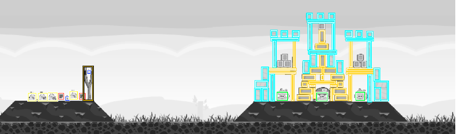
\includegraphics[width=150mm]{level.png}
\end{center}
\caption{Ausschnitt aus Level 21 Angry Birds}
\small
Das Bild zeigt ein Level aus Angry Birds mit einer komplizierten Struktur, die aus verschiedenen Objekten mit unterschiedlichen Eigenschaften besteht, hier dargestellt durch Bounding-Boxen.
\end{figure}

Aus Sicht von Künstlicher Intelligenz vereint das Spiel Aspekte aus den Bereichen Computer Vision, Maschinelles Lernen, Wissensrepräsentation, Planen, Heuristische Suche und Schlussfolgern unter Unsicherheit \cite{renz2015aibirds}. Einen intelligenten Agenten für dieses Spiel zu entwickeln, der besser sein soll als menschliche Spieler, ist genau deshalb für die Forschung von gro\ss er Bedeutung und stellt das Team vor schwierige Herausforderungen.